\chapter{Benchmarking Personal Clouds Synchronization}

In the evaluation of the reference implementation of StackSync framework, we set out to answer three basic questions: 
$1$) \textit{How much overhead does the system need to support?} $2$) \textit{How much time is needed to have multiple devices in sync?}; and 
$3$) \textit{How does the system internally scale?}

In some of these tests, we compare StackSync against other popular Personal Cloud services, including Dropbox, Microsoft OneDrive, Amazon Cloud Drive, Google Drive and Box.

\section{Benchmark Methodology}

\subsection{Benchmark Testbed}

For all the experiments, we used the following testbed. The testbed included a front-end server and several desktop 
PCs acting as clients. The front-end was an OpenStack Swift deployment with one proxy node and $4$ storage nodes.  
Unless otherwise noted, the proxy node hosted the \texttt{SyncService}, and the PostgreSQL database acting as the \texttt{Metadata back-end}. Let us review the node specs:
\begin{itemize}
\item Proxy node: Ubuntu $12.04$; Intel Xeon CPU E5-2407; Memory: $12$ GB RAM.
\item Storage nodes: Ubuntu $12.04$;  Intel Xeon CPU E5-2403; Memory: $8$ GB RAM.
\item Desktop PCs: Ubuntu $12.04$; Intel Core i5 2400; Memory: $4$ GB RAM.
\end{itemize}

Tables~\ref{table:services} and~\ref{table:clients} shows the software versions for the services and desktop clients used in the evaluation.

\begin{table}[!htb]
    \begin{minipage}{.5\linewidth}
      \centering
        \begin{tabular}{ | l | l | }
    	\hline
    	Service name & Version \\ \hline
    	OpenStack Swift & \textit{Havana} \\
    	RabbitMQ & 2.8.7 \\
    	PostgreSQL & 9.1 \\
    	SyncService & 0.4.4 \\ \hline
    	\end{tabular}
    \caption{Used services version}
    \label{table:services}
    \end{minipage}%
    \begin{minipage}{.5\linewidth}
      \centering
        \begin{tabular}{ | l | l | }
    	\hline
    	Client name & Version \\ \hline
    	StackSync & 1.6.4 \\
    	Dropbox & 2.6.33 \\
    	Microsoft OneDrive & 17.0.4035.0328 \\
    	Amazon Cloud Drive & 2.4.2013.3290 \\ 
    	Google Drive & 1.15.6430.6825 \\ 
    	Box & 4.0.4925 \\ \hline
    	\end{tabular}
    \caption{Used desktop clients version}
    \label{table:clients}
    \end{minipage} 
\end{table}

\subsection{Setup and Benchmarking Tool}

To evaluate the system, we developed a benchmarking tool to generate
realistic workloads. We implemented this tool because we found no publicly available trace containing both 
the files and the history of modifications to those files that allowed us to evaluate our file-syncing service.

To determine the size of the files, we used the distribution presented in~\cite{liu2013},
a five-month study involving around $20,000$ users. Some of their conclusions
were that the $90\%$ of files are smaller than $4$ MB and that updated files tend to be read sooner
rather than later. Also, they noticed that most of files are read-only.

Imitating the real behavior of users, our tool creates a trace with $3$ different actions: ADD representing the addition
of a file, UPDATE signaling a modification, and REMOVE meaning the removal of the file from the workspace.

In order to determine the action to be performed to a file, we applied the Markov model proposed in~\cite{Tarasov12}. 
In this model, each file can be in $4$ possible states: $\mathtt{N}$ \textemdash~new; $\mathtt{M} $\textemdash~modified; 
$\mathtt{U}$ \textemdash~unmodified; and $\mathtt{D}$ \textemdash~deleted.
For each of those states, a set of probabilities govern the transition to the rest of states.
To set up the transition~probability
matrix, we extracted the transition probabilities from the ``\textit{Homes}'' dataset~\cite{Tarasov12}, 
which is the public trace that most resembles the user behavior in a Personal Cloud service.

To decide how to modify the files, we followed the same approach as in \cite{Tarasov12},
which currently supports $3$ modification types: $\mathtt{B}$ \textemdash~the file is modified in the
beginning by prepending some bytes; $\mathtt{E}$ \textemdash~the file is modified at the end; and $\mathtt{M}$ \textemdash~the
file is modified somewhere in the middle.  As in \cite{Tarasov12}, we also supported
combinations of these patterns, namely $\mathtt{BE}$, $\mathtt{BM}$, and $\mathtt{EM}$. For the transition 
probabilities, we used the change pattern of the ``\textit{Homes}'' dataset: the probability for a $\mathtt{B}$ 
change was of $38\%$; for a $\mathtt{E}$ change was of $8\%$, and for a $\mathtt{M}$ change was of $3\%$. 
The rest of the probability mass was granted to combinations of these changes. We only applied these probabilities
in files smaller than $4$ MB, since more than $90\%$ of the I/O requests are for these files, as just
discussed above.

Our trace generator requires only $3$ parameters: $1$) initial number of files; $2$) number
of training iterations; and $3$) number of snapshots. For our experiments, we set the
initial number of files to $20$, and the number of iterations and snapshots to $5$ and
$100$, respectively. The resulting trace contained $940$ ADDs, $72$ UPDATEs and $228$ REMOVEs.
The ADD operations generated a total data volume of $535.41$ MB whereas the UPDATEs only produced
$\approx 14$ KB. The average file size was of $583$ KB. Fig.~\ref{fig:cdf_files} plots
the CDF of file size for our trace.

Finally, to compare StackSync, our open source Personal Cloud, against other popular Personal Cloud services,
we modified the benchmarking tool developed by Drago et al.~\cite{drago2013benchmarking} to
conduct trace-driven experiments with the output of our generator. More specifically, we adapted
their tool to measure the overhead of the different file syncing protocols under a sequence of
ADD, UPDATE, and DELETE operations using real content.

\begin{figure*}[t]
  \centering
  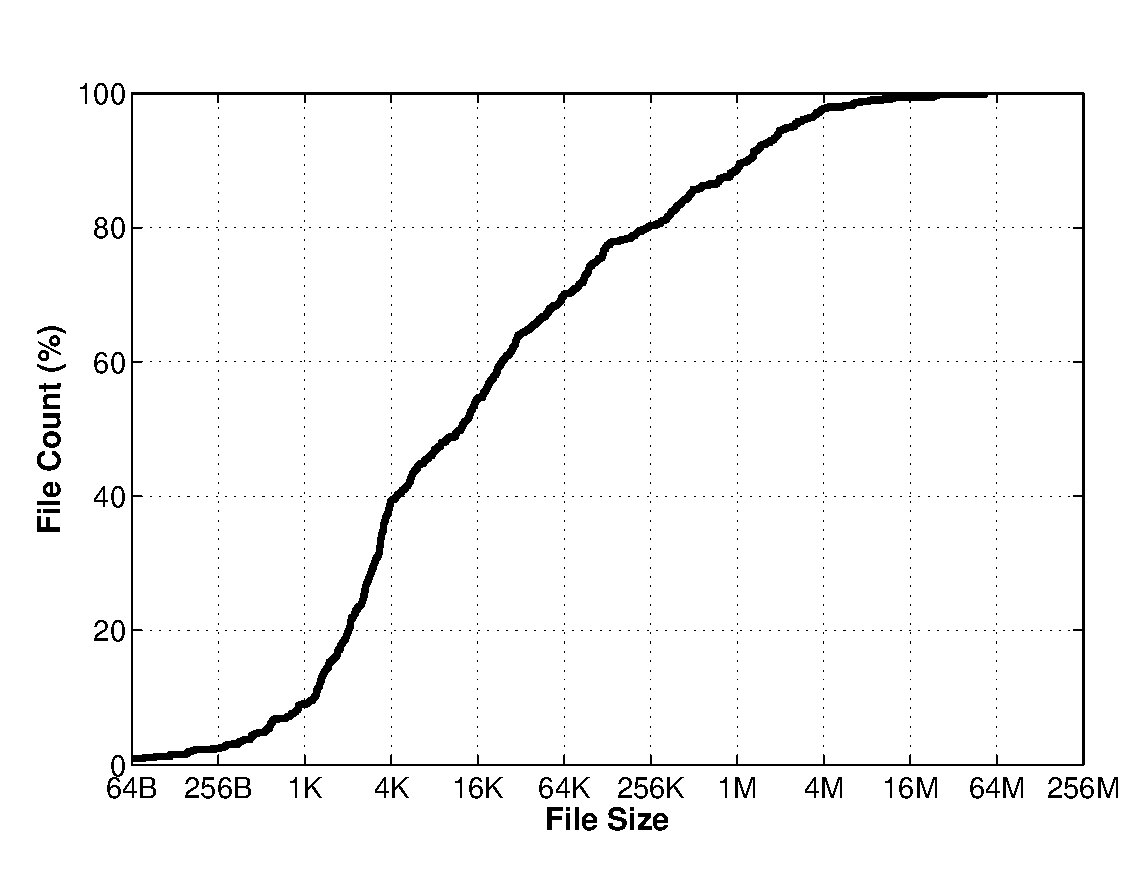
\includegraphics[width=0.7\textwidth]{figures/cdf_files}
  %\vspace{-5pt}
  \caption{File size vs file count distribution}
  \label{fig:cdf_files}
\end{figure*}

\section{Results}

\subsection{Protocol Overhead}
In this test, we compared the protocol overhead of StackSync with the overhead of the
commercial Personal Cloud services reported in Table~\ref{table:clients}. As in~\cite{drago2013benchmarking},
we defined the overhead as the total storage and control traffic over the benchmark size, which was of 
$535.41$ MB. For this experiment, our benchmarking tool considered each of the operations in the trace one at a time,
to measure the overhead accurately. That is, the next operation did not start until the current one was
successfully committed.

\begin{figure*}[h]
  \centering
  \label{fig:overhead_clients}
  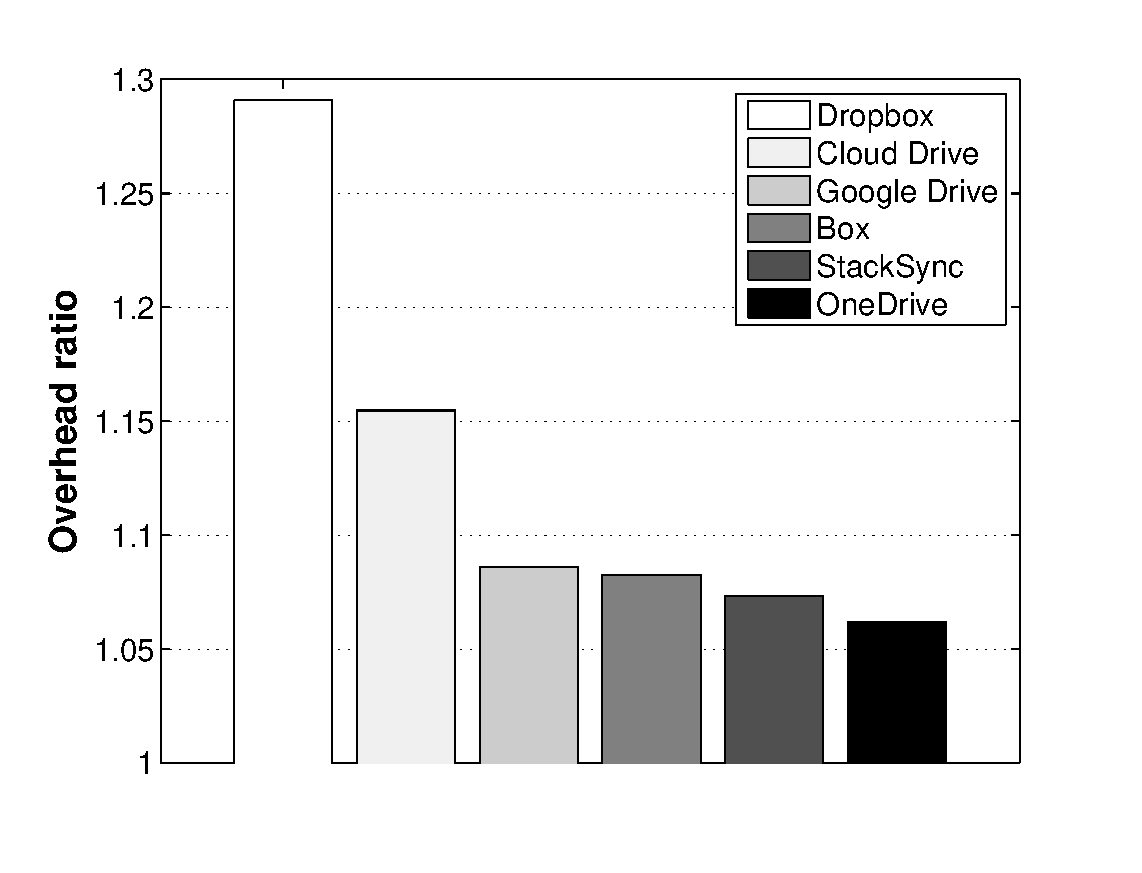
\includegraphics[width=0.6\textwidth]{figures/overhead_clients}
  \caption{Overhead}
\end{figure*}

The results are shown in Fig.~\ref{fig:overhead_clients}. As seen in this
figure, Dropbox exhibits the highest overhead, sending up to $150$ MB of additional
unnecessary traffic. This results agree very well with other studies such as that
of~\cite{liu2013}. On the contrary, StackSync has a low overhead, \textit{comparable to that of commercial
Personal Cloud services such as OneDrive}.


To gain a deeper understanding of the overhead, we prepared a new variant of
this test. In this new variant, we grouped all the actions of the same type to generate $3$ separate traces,
and this way study the overhead per type of action. In this case, we run this experiment only for Dropbox and StackSync
for two main reasons: $1$) because 
Dropbox is the most popular and well-studied Personal Cloud; and $2$) because
it is the Personal Cloud with the highest overhead, which allows for rapid comparison. 
The results are depicted in Fig.\ref{fig:validation:actions_control} for control traffic and Fig.\ref{fig:validation:actions_storage}
for storage traffic.

As shown in Fig.\ref{fig:validation:actions_control}, Dropbox produces a huge amount of control traffic
when adding new files, about $25$ MB of unnecessary traffic, while StackSync only needs $\approx 3.2$ MB.
This indicates that control signaling is significantly much lighter than that of Dropbox. With respect
to storage traffic, StackSync transferred a total amount of $565.63$ MB to the \texttt{Storage back-end},
which is significantly smaller than the $660.32$ MB of storage traffic incurred by Dropbox.

For the UPDATEs, StackSync is negatively affected by the fact that a modification of a few bytes requires to upload at 
least one chunk of  $512$ KB, incurring a huge overhead. Since Dropbox uses delta encoding~\cite{drago2013benchmarking}, a specialized
compression technique, it outperformed StackSinc. It is important to note here that although the 
overhead for StackSync is apparently high, in practice, StackSync transferred only $5$ MB and Dropbox $2$ MB. 
Both values are relatively high compared with the amount of  modified data ($13.50$ KB). 

As the setup of these tests were not favorable to Dropbox, because the actions were performed one after
another without benefiting from the Dropbox file bundling feature, we created a new test that
performs more one action at the same time. Table \ref{table:bundle} lists
the results obtained after executing the trace for both Dropbox and StackSync with different
batch sizes. Dropbox reduces traffic overhead in $30$ MB but it continues to be much higher than the
rest of the Personal Clouds.

\begin{figure*}[t]
  \centering
  \subfigure[Control traffic overhead]{
    \label{fig:validation:actions_control}
    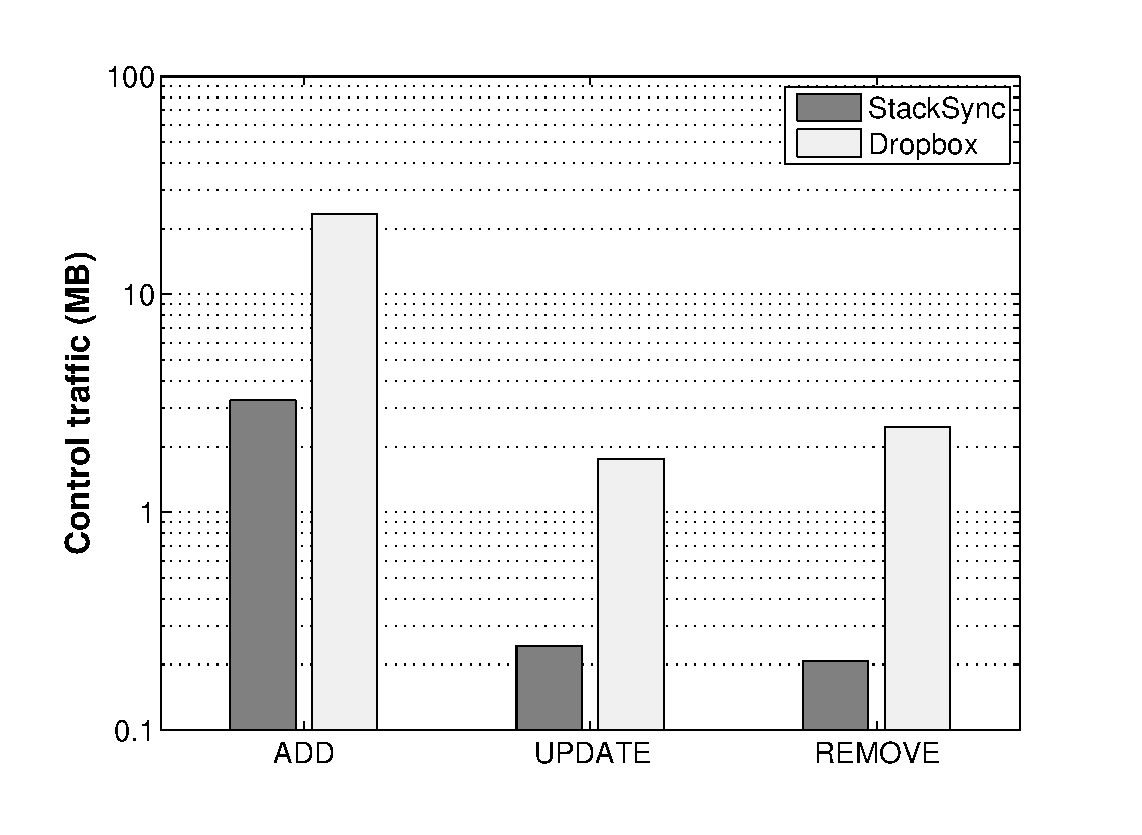
\includegraphics[width=0.45\textwidth]{figures/actions_metadata}
  }
  \subfigure[Storage traffic overhead]{
    \label{fig:validation:actions_storage}
    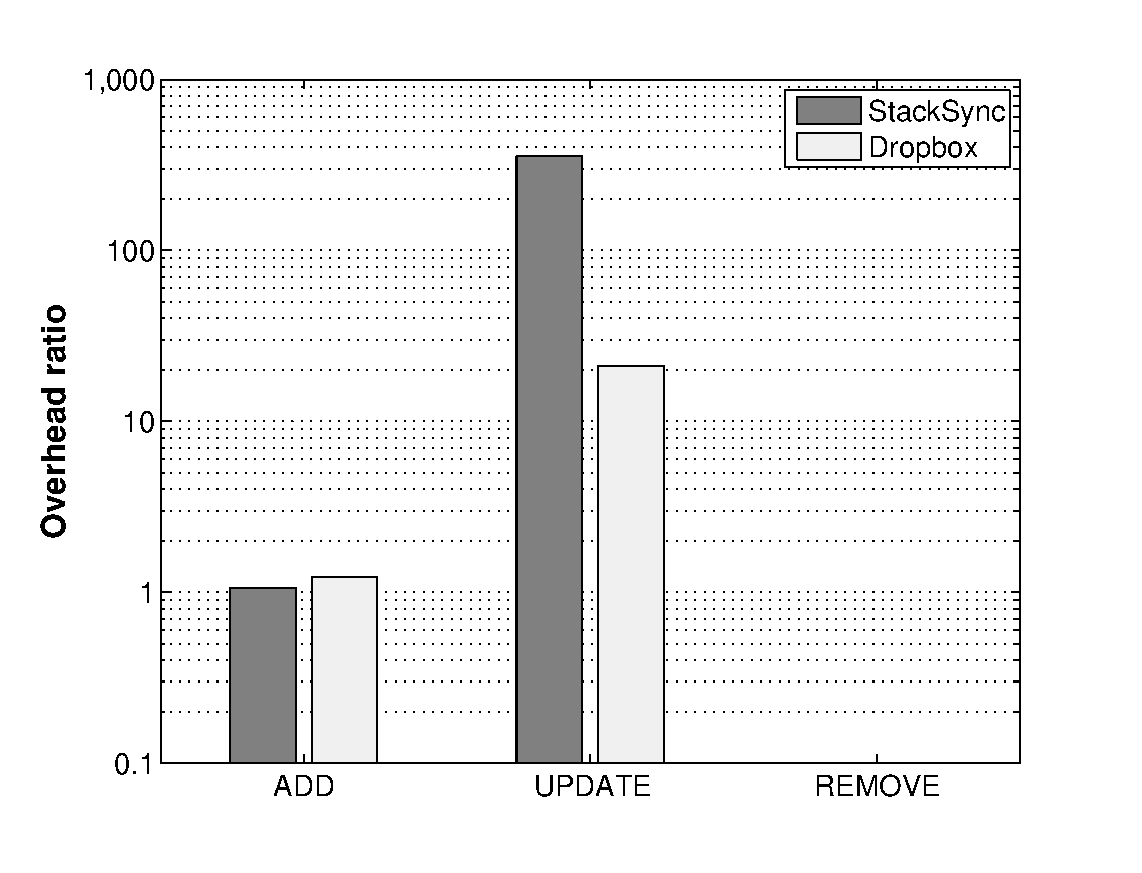
\includegraphics[width=0.45\textwidth]{figures/actions_storage}
  }
  \caption{Control and storage traffic overhead of StackSync and Dropbox}
  \label{fig:validation}
\end{figure*}

\begin{table}
    \centering
    \begin{tabular}{  c | c | c | c | c | }
    \cline{2-5}
    & Batch size & Control & Storage & Total \\ \hline
    \multicolumn{1}{ |c| }{\multirow{4}{*}{Dropbox}} & 5 & 8.30 MB & 633.06 MB & 641.36 MB \\ \cline{2-5}
    \multicolumn{1}{ |c| }{}& 10 & 5.13 MB & 638.26 MB & 643.39 MB \\ \cline{2-5} 
    \multicolumn{1}{ |c| }{}& 20 & 3.28 MB & 635.82 MB & 639.10 MB \\ \cline{2-5}
    \multicolumn{1}{ |c| }{}& 40 & 2.23 MB & 632.05 MB & 634.28 MB \\ \hline
    \multicolumn{1}{ |c| }{\multirow{4}{*}{StackSync}} & 5 & 2.14 MB & 569.89 MB & 572.03 MB \\ \cline{2-5}
    \multicolumn{1}{ |c| }{}& 10 & 1.58 MB & 570.10 MB &  571.68 MB \\ \cline{2-5}
    \multicolumn{1}{ |c| }{}& 20 & 1.37 MB & 570.07 MB & 571.44 MB \\ \cline{2-5}
    \multicolumn{1}{ |c| }{}& 40 & 1.25 MB & 567.77 MB & 569.02 MB \\ \hline
    \end{tabular}
    \caption{Effect of File Bundling.}
    \label{table:bundle}
\end{table} 

\subsection{Synchronization Time}

Another basic question to be examined is the delay experienced~by users to have their devices in sync. 
To answer this question, we measured the time to synchronize $6$ clients for each type
of workspace changes, i.e., ADD, UPDATE and REMOVE. 
The synchronization time was measured as the time elapsed after the modification
was detected by the \texttt{Watcher} of the client that performed it until the local working copies of the other
five clients were in sync. In the case of ADDs and UPDATEs, this time included the delay incurred
to upload and download the unique chunks from the \texttt{Storage back-end}, hosted in our local cluster. 

The results are depicted in Fig.~\ref{fig:synchronization_time:a}. As can be seen in the figure, all the operations take
only a few seconds to have all the clients in sync, even in the case of the ADD operation where an appreciable
amount of time is taken up to access the \texttt{Storage back-end}. Because the REMOVE operation does not trigger any data flow to and from the
\texttt{Storage back-end}, the synchronization time becomes a good estimator of the processing time
incurred by the tandem ObjectMQ-\texttt{SyncService}. 

As shown in the figure, the time to reconcile
a file removal in five clients is less than $2.6$ seconds, which is quite good, assuming that the
\texttt{Metada back-end} is a SQL database.
As a boxplot enables to assess the dispersion of a given distribution, 
we gain important qualitative
insights from Fig.~\ref{fig:synchronization_time:a}. One key observation is that the distribution of the
synchronization time for the UPDATE operation is right skewed, exhibiting file synchronization times
significantly greater than the median value of $2.75$ seconds. This is evidenced~by
the significant number of UPDATE operations exceeding the upper whisker. This skewness is explained
by the use of fixed-size blocks, which suffer from the \textit{boundary shifting problem}~\cite{Eshghi05}.

Since the time taken up by the ADD operation is affected by the file size, one interesting question
is to assess how file size affects the synchronization time. Fig.~\ref{fig:synchronization_time:b} shows the synchronization
time as a function of file size. As can be seen in the figure, \textit{the larger the file size, the longer
the synchronization time}. However, what is most interesting is the fact that the increase in time
is only linear when file size is larger than $2.5$ MBs, which indicates that for small files the
time to transfer chunks from and to the \texttt{Storage back-end} is not significant compared
with the time incurred by the tandem ObjectMQ-\texttt{SyncService}. 

\begin{figure*}[t]
  \centering
  \subfigure[Boxplots of synchronization time]{
    \label{fig:synchronization_time:a}
    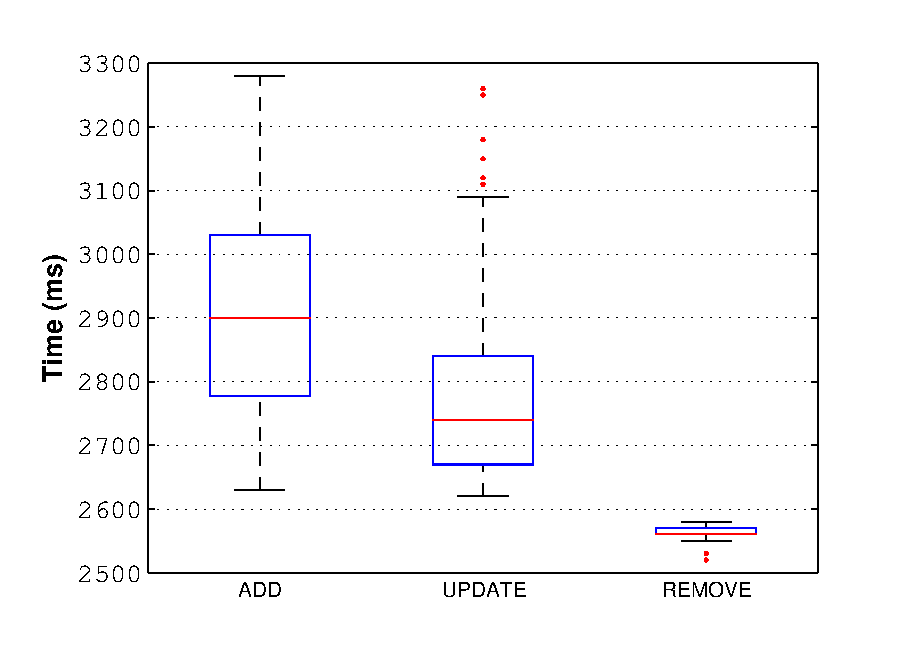
\includegraphics[width=0.45\textwidth]{figures/fig10_2}
  }
  \subfigure[Synchronization time against file size]{
    \label{fig:synchronization_time:b}
    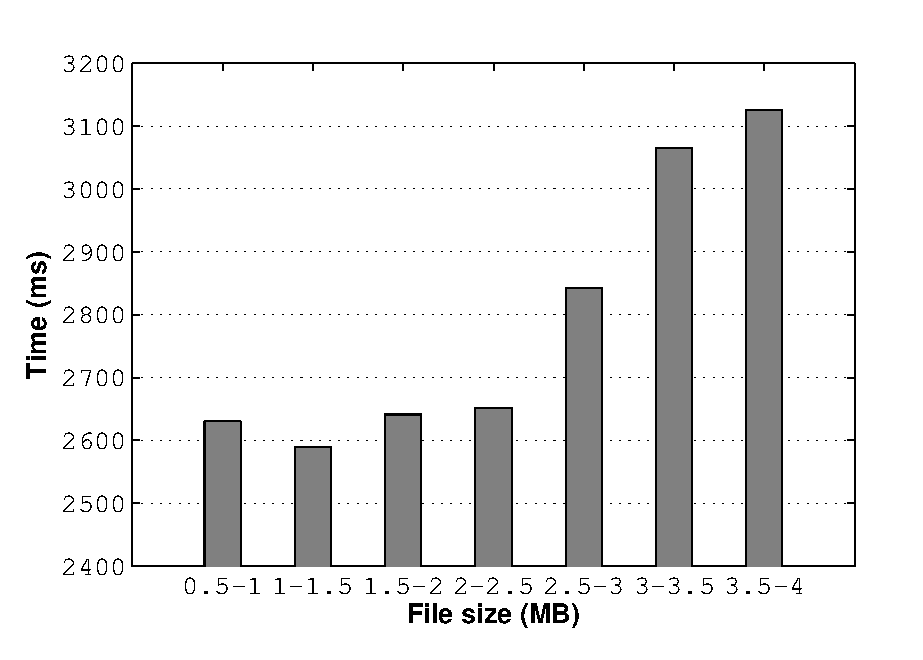
\includegraphics[width=0.45\textwidth]{figures/fig11}
  }
	\caption{Synchronization time}
  \vspace{-5pt}
  \label{fig:synchronization_time}
\end{figure*}


\subsection{Scalability and load-balancing}

Finally, we performed an initial experiment to assess the scalability and load-balancing of 
the StackSync platform. To this end, we performed stress tests generating $100$, $200$, and
$400$ commit requests per second from different clients. We wanted to measure how our service
handles a high number of operations per second, and how the load can be balanced among different
\texttt{SyncService} instances.

In this experiment, we used several system setups: $10$ Desktop PCs generating each one $10$ 
requests per second ($100$ commits/sec in the server), $20$ Desktop PCs generating each one
$10$ requests per second ($200$ commits/sec in the server), and $20$ Desktop PCs generating
each one $20$ requests per second ($400$ commits/sec in the server). 
The used trace was the same of the prior experiments but injected from different clients.
For each system configuration, we executed the experiment using either one single-threaded or four single-threaded 
\texttt{SyncService} instances. 

For each commit request, we recorded the time since the client sent out the commit request until the commit event 
confirming this changes was received in the client. Note that this time captured the entire life-cycle of the protocol,
including message dispatching, time to process the operation in the \texttt{SyncService}
(including access to the database), and finally the dispatching of the commit event to the requesting node.

\begin{figure}[t]
\centering
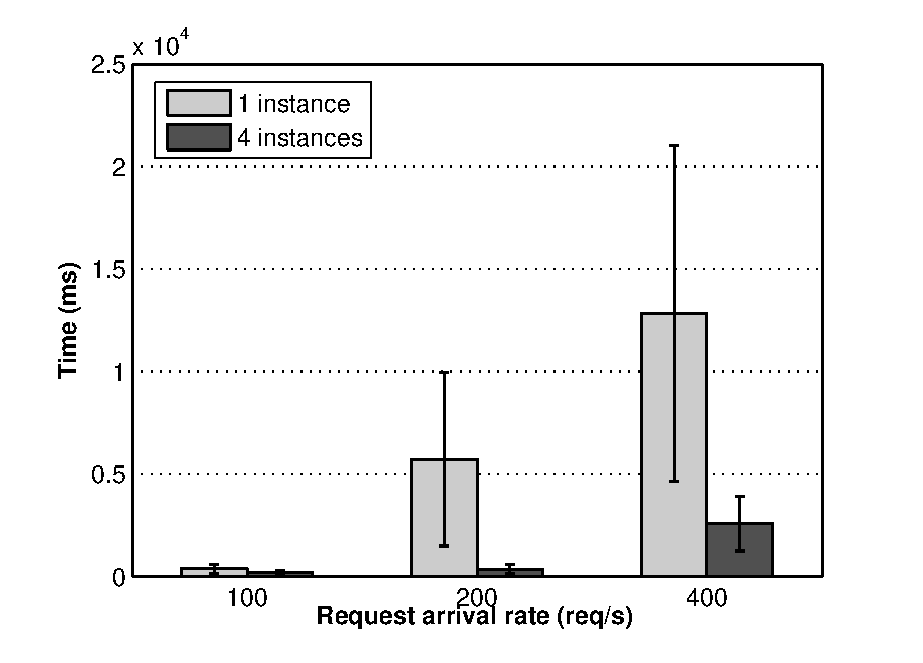
\includegraphics[width=0.5\textwidth]{figures/performance_scalability}
\caption{Scalability and load balancing}\label{fig:scalability}
\end{figure}


In Fig. ~\ref{fig:scalability}, we illustrate the time for $1$ and $4$ \texttt{SyncService}s under different
loads: $100$, $200$, $400$ commits/sec. Our service shows promising numbers in the processing of concurrent
requests since it is able to handle a commit in less than $0.1$ seconds with $4$ instances when receiving
a bulk of $200$ requests/sec. This clearly indicates that balancing the load
among multiple instances produces a significant performance boost. If we consider that all services are
running in the same machine, our results show that the bottleneck is in the transactional database
rather than in the communication layer, i.e., ObjectMQ. The performance gains observed here open the
way to future optimizations to fine tune the scalability of the overall service. 





\subsection{ownCloud Vs StackSync}

In this first experiment we want to compare the metadata overhead produced by ownCloud and StackSync. As stated in the related work, ownCloud is using a pull-based approach based on the WEBDAV protocol. The ownCloud client discover changes by continuously pulling the server with WEBDAV PROPFIND requests for the root user folder every 30 seconds approximately. Each of these requests returns a XML file with a full list of the files and their associated metadata.


Since the PROPFIND request only returns the metadata of the files in the same level, it will not contain change information of files or folders in the levels below. This implies that a change in a subfolder will trigger recursive PROPFIND requests in all the levels of the path. When the change is located in the subfolder, the client then performs a GET request to retrieve the file and stay synced with the rest of the clients.

Due to obvious reasons, this behaviour can be highly inefficient since the amount of metadata exchanged between the server and the client to stay synced could be important (i.e. discover a new file stored in a five-level depth folder produces five PROPFIND requests). It is also important to take into account that each PROPFIND request over a folder involves to get the metadata of all the files inside this folder.

In Fig.~\ref{fig:owncloud} we can see the metadata overhead for ownCloud and StackSync when one node modifies files (uploader) and other must synchronise these changes (downloader). As we can observe in the figure, ownCloud's uploader node is producing for our experiment around 600-800 KBytes/minutes of metadata traffic, and the downloader is producing around 100-300 KBytes/minute of medatada traffic.  This massive traffic is a direct consequence of the inefficient ownCloud pull protocol.

In Fig.~\ref{fig:owncloud} we can see the sequence diagram of ownCloud sync protocol. The node committing new changes (uploader) first obtains the current state (PROPFIND), then uploads the file (PUT), then requests the new change (PROPPATCH), and then rechecks with PROPFIND that the change was correctly applied. The rest of nodes (downloaders) will just ask for changes (PROPFIND) and then retrieve (GET) the entire file. 


Note that PROPFIND and PROPPATCH are synchronous calls that are blocking the client and the server. Note also that if the change is not located in the root folder, it will require recursive PROPFIND requests for the entire path to the change for all clients.  This is not an optimized protocol but a simple pull interface to WEBDAV. As we can see in Fig.~\ref{fig:owncloud},  StackSync is producing an order of magnitude less overhead  than ownCloud for the same experiment  (around 10KBytes/Minute for both uploader and downloader nodes). 


Besides the inefficient metadata processing based on WebDAV pulling, data traffic is coupled to the same metadata server. Furthermore, ownCloud lacks any chunking, deduplication or even caching mechanisms. It just uploads or downloads the entire file if anything has changed.

ownCloud has devoted most efforts in developing the web document manager and web applications. They are providing a very simple and minimalist WEBDAV front-end  to their web server. This could work for a single user (home repository) but the amount of useless traffic make it clearly infeasible for a large deployment.

\begin{figure*}[t]
  \centering
  \subfigure[ownCloud vs StackSync metadata overhead]{
    \label{fig:time:a}
    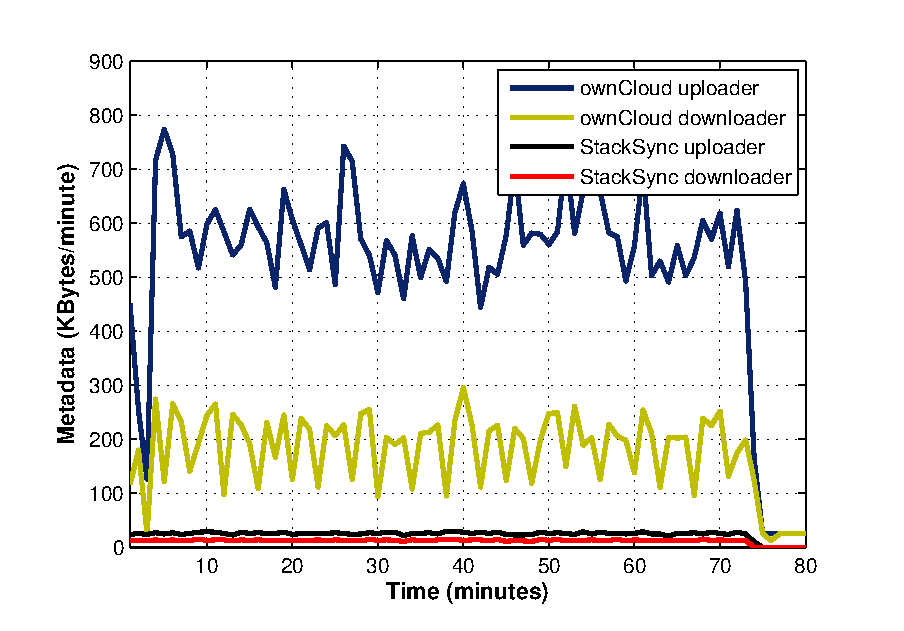
\includegraphics[width=0.45\textwidth]{figures/owncloud_vs_ss_metadata}
  }
  \subfigure[ownCloud sync protocol]{
    \label{fig:time:b}
    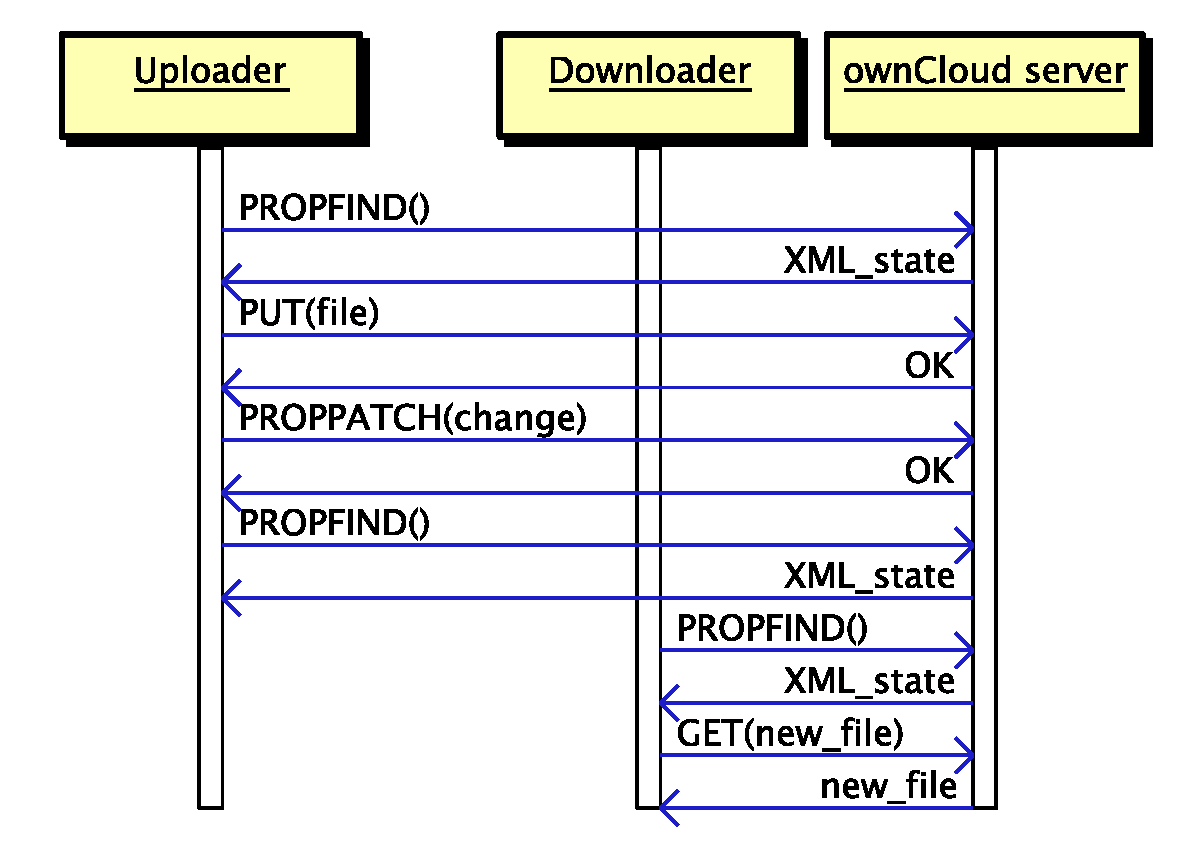
\includegraphics[width=0.45\textwidth]{figures/owncloud}
  }
  \caption{ownCloud vs StackSync}
  \vspace{-5pt}
  \label{fig:owncloud}
\end{figure*}